% n=3 coupon collection: the probabilities and means at successive stages are exact.
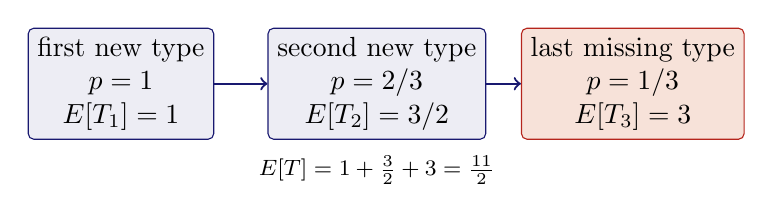
\begin{tikzpicture}[x=1cm,y=1cm,line cap=round]
  \node[draw=MidnightBlue,fill=MidnightBlue!8,rounded corners=2pt,minimum width=2.25cm,minimum height=1.25cm,align=center] (one) at (0,0) {first new type\\$p=1$\\$\mathbb E[T_1]=1$};
  \node[draw=MidnightBlue,fill=MidnightBlue!8,rounded corners=2pt,minimum width=2.25cm,minimum height=1.25cm,align=center] (two) at (3.25,0) {second new type\\$p=2/3$\\$\mathbb E[T_2]=3/2$};
  \node[draw=BrickRed,fill=BrickRed!10,rounded corners=2pt,minimum width=2.25cm,minimum height=1.25cm,align=center] (three) at (6.5,0) {last missing type\\$p=1/3$\\$\mathbb E[T_3]=3$};
  \draw[->,MidnightBlue,thick] (one.east)--(two.west);
  \draw[->,MidnightBlue,thick] (two.east)--(three.west);
  \node[font=\footnotesize] at (3.25,-1.1) {$\mathbb E[T]=1+\frac32+3=\frac{11}{2}$};
\end{tikzpicture}
